  \section{Implementasi Perangkat Lunak}
  Pada subbab ini, penulis akan memaparkan mengenai spesifikasi dan pemasangan perangkat lunak yang dibutuhkan dalam rancang bangun aplikasi lelang online ini.
  
  \subsection{Arsitektur Perangkat Lunak}
  \label{arsitektur-pl-final-subbab}
	  Arsitektur aplikasi saat ini dapat dijelaskan lewat diagram berikut
	  
	  
	  
	  
  
  \subsection{Pemasangan \& Konfigurasi Perangkat Lunak}
	  Pada subbabb ini, penulis menuliskan tahap-tahap pemasangan dan konfigurasi untuk komponen-komponen yang ada di subbab \ref{arsitektur-pl-final-subbab}.
	  
	\subsubsection{\textsc{Nginx}}

\begin{enumerate}
	\item CORS (\textit{Cross Origin Resource Sharing})
	\\
	CORS adalah sebuah mekanisme yang memungkinkan  sebuah \textit{website} menggunakan \textit{resources}(seperti skrip Javascript, \textit{fonts}, dll) untuk diakses dari sumber lain selain \textit{domain origin}nya.Secara teknis, CORS mendefinisikan \textit{protokol}/cara browser dan server untuk berinteraksi otorisasi permintaan \textit{resource} dari domain lain, dan juga lebih aman karena \textit{developer} dapat mengkontrol otorisasi tersebut (daripada mengizinkan semua permintaan).\\
	
	% todo cite wikipedia
	\textbf{\textit{The Problem}} \\
	Masalah koneksi ke server lelang (yang berjalan pada domain yang sama, namun port yang berbeda) tidak dapat tersambung karena \textit{error} berikut :


	\begin{figure}[H]
		\centering
		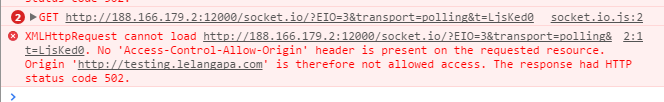
\includegraphics[width=\textwidth]{images/bab4/pl/madafaka_cors.png}
		\caption{\textit{Error} CORS yang muncul pada console browser}
		\label{cors}
	\end{figure}
	
	
	\textbf{\textit{Insight}} \\
	Selama 2 minggu kurang lebih penulis mencoba cara yang ditemukan penulis dalam situs stackoverflow untuk mengkonfigurasi \textit{server} lelang agar otorisasi CORS dapat dilakukan, namun tidak ada hasil.\\
	\indent Masalah ini terselesaikan setelah menggunakan fitur \textit{reverse proxy} dari Nginx.\\
	
	\textbf{\textit{Solution}} \\
	\indentenum Strateginya adalah sebagai berikut :
	\begin{enumerate}
		\item \label{nginx-a} \textit{Server} lelang berjalan pada localhost port 3000.
		\item \label{nginx-b} Diatur sebuah subdomain khusus -- misalkan A.domain.com
		\item \textsc{Nginx} dikonfigurasi dimana semua \textit{requests} menuju A.domain.com ke aplikasi \textit{localhost} yang kita maksud di poin \ref{nginx-a}
		\item Selain meneruskan \textit{requests}, \textsc{Nginx} juga akan meneruskan \textit{reply} dari server lelang tersebut kepada \textit{client}/\textit{origin} yang meminta \textit{request} tersebut.				
	\end{enumerate}
\end{enumerate}
	\input{Chapters/Details/bab4/4b/laravel}
	\input{Chapters/Details/bab4/4b/postgre}
	\input{Chapters/Details/bab4/4b/mongo}
	\subsubsection{\textsc{Vue.js}}
	% todo inline numbering
	
\begin{enumerate}
\item \textbf{\textit{Package Dependencies}} \\
	Pada versi terbaru Laravel (5.4*), Laravel secara \textit{default} menyertakan \textit{package} Laravel Mix - yaitu fitur untuk \textit{compiling assets} dengan Webpack, dengan hasil akhir \textit{compiled assets} (terutama \textit{script} Javascript) yang eksekusinya jauh lebih cepat, karena menggunakan V8 -- sebuah \textit{engine} Javascript yang telah dioptimasi yang bersifat \textit{just-in-time} (JIT) yang memproduksi \textit{machine code} dari sebuah \textit{script} Javascript lalu dieksekusi.\\
  
  \textbf{\textit{Main Problem}} \\
  Masalah muncul saat versi Laravel yang digunakan untuk membangun aplikasi adalah versi (5.3) -- dan jika Laravelnya di\textit{upgrade}, tidak ada jaminan bahwa \textit{deprecated dependencies} (keadaan dimana sebuah \textit{package} tidak di\textit{support} oleh versi terbaru) -- yang berarti harus \textit{refactoring code} yang pasti memakan waktu lama.\\			  

	\textbf{\textit{Insights}} \\
	Penulis menganalisa perbedaan mendasar package.json antara Laravel 5.3 dan 5.4 adalah sebagai berikut:
	\begin{enumerate}[label={\alph*}.]
  	  	\item Basis : Perubahan basis yang awalnya Gulp menjadi Webpack
  	  	\item \textit{Dependencies} : Webpack ternyata menggunakan beberapa plugin tambahan yang tidak diakomodasi dalam package.json di versi 5.3
  	  	\item \textit{Run Script} : Terdapat beberapa perubahan signifikan terhadap \textit{run script alias} di versi 5.4 - dibandingkan pada versi 5.3.
  	  	\item \textit{Additional Files} : Terdapat beberapa file konfigurasi tambahan agar proses kompilasi aset dapat berjalan dengan baik.
	\end{enumerate}
	\ \\
  
  \textbf{\textit{Solution}} \\
  Penulis lalu mengoreksi dan \textit{update package.json} dengan pendekatan \textit{trial and error}, dan bisa terselesaikan dengan script berikut :
	\begin{lstlisting}[language=json]
{ "private": true,
  "scripts": 	{
	"_comment" : "Lists of running npm commands defined here"
  },
  "devDependencies": {
	"axios": "^0.15.3",
	"bootstrap-sass": "^3.3.7",
	"cross-env": "^3.2.3",
	"jquery": "^3.1.1",
	"laravel-mix": "0.*",
	"lodash": "^4.17.4",
	"vue": "^2.1.10"
  },
  "dependencies": {
	"vue-resource": "^1.3.1"
  } }
\end{lstlisting}	  	

			  	
	\ \\		  
\item 
	\textbf{\textit{Dependencies Optimization}} \textbf{\textit{Problem}} \\
	Setelah menulis beberapa \textit{script} Vue, penulis menganalisa bahwa setiap \textit{script} Vue ternyata mempunyai \textit{dependencies} yang sama, yaitu axios, Promise, toastr dan vue. Setiap file Vue meng\textit{include} sebuah \textit{script} yang berisi:
	\begin{lstlisting}[style=htmlcssjs]
	window.axios = require('axios');
	window.toastr = require('toastr');
	window. = require('toastr');
	require('vue-resource');
\end{lstlisting}

	Hal ini mengakibatkan semua file vue yang di\textit{compile} ukurannya cukup besar (~400KB), padahal sebenarnya di dalam setiap file tersebut sebenarnya ada yang sama. Hal ini tentu tidak efektif, karna sebenarnya hal-hal yang sama tersebut bisa dipisahkan, dan dijadikan \textit{cache} sehingga \textit{loading} halaman bisa jauh lebih cepat.\\
		
	\textbf{\textit{Insight \& Solution}} \\
	Setelah penulis berdiskusi di forum Slack, beberapa pengguna Vue menyarankan untuk \textit{compile} keseluruhan \textit{dependencies} yang digunakan kedalam satu file terpisah, dan hanya menulis logika Vue untuk setiap file Vue.\\
	Isi file webpack.mix.js (file yang di\textit{compile} oleh Webpack)	menjadi seperti berikut.
	
\begin{lstlisting}[style=htmlcssjs]
/* dependencies all compiled into one single file */
mix.js('scripts/dependencies.js', 'public/js');

/* dependencies all compiled into one single file */
mix.js('scripts/favorites.js', 'public/js');
mix.js('scripts/other_vue_script.js', 'public/js');
\end{lstlisting}
		
	Dan di HTML, untuk \textit{including} \textit{script} dituliskan seperti berikut:
	\begin{lstlisting}[style=htmlcssjs]
<script src="dependencies.js" ></script>
<script src="custom_page_script.js" ></script>
\end{lstlisting}

\end{enumerate}
	\input{Chapters/Details/bab4/4b/node}
	\input{Chapters/Details/bab4/4b/socketio}
	\subsubsection{Instalasi \textsc{JWT} pada Laravel dan Node.js}
	\subsubsection{\textsc{SendGrid Whitelisting}}
	% todo inline numbering

	\subsubsection{Instalasi \& Konfigurasi \textbf{Amazon Web Service S3}}

	\begin{enumerate}[label={}]
		
		\item \textbf{Instalasi \textbf{AWS}} 
			\\Tahap-tahap untuk instalasi adalah sebagai berikut
			\begin{enumerate}[label=\roman*]				\item \mylipsum
					\begin{figure}[H]
						\centering
						
\includegraphics[width=0.4\textheight]{images/no-image.png}
						\caption{Skrinsut Tahap 1 Instalasi \textbf{AWS}}
						\label{pdm-final}
					\end{figure}				\item \mylipsum
					\begin{figure}[H]
						\centering
						
\includegraphics[width=0.4\textheight]{images/no-image.png}
						\caption{Skrinsut Tahap 2 Instalasi \textbf{AWS}}
						\label{pdm-final}
					\end{figure}		
						
			\end{enumerate}
		\item 
		\textbf{Konfigurasi \textbf{AWS}}
		\begin{enumerate}[label=\roman*]
			\item \mylipsum
			\begin{figure}[H]
				\centering
				
\includegraphics[width=0.4\textheight]{images/no-image.png}
				\caption{Skrinsut Tahap 1 Konfigurasi \textbf{AWS}}
				\label{pdm-final}
			\end{figure}					
			\item \mylipsum
			\begin{figure}[H]
				\centering
				
\includegraphics[width=0.4\textheight]{images/no-image.png}
				\caption{Skrinsut Tahap 1 Konfigurasi Nginx \textbf{AWS}}
				\label{pdm-final}
			\end{figure}	
	 	\end{enumerate}
	\end{enumerate}
	
	 
  
  
  
  
  
  
